%%
%% This is file `sample-sigconf.tex',
%% generated with the docstrip utility.
%%
%% The original source files were:
%%
%% samples.dtx  (with options: `all,proceedings,bibtex,sigconf')
%% 
%% IMPORTANT NOTICE:
%% 
%% For the copyright see the source file.
%% 
%% Any modified versions of this file must be renamed
%% with new filenames distinct from sample-sigconf.tex.
%% 
%% For distribution of the original source see the terms
%% for copying and modification in the file samples.dtx.
%% 
%% This generated file may be distributed as long as the
%% original source files, as listed above, are part of the
%% same distribution. (The sources need not necessarily be
%% in the same archive or directory.)
%%
%%
%% Commands for TeXCount
%TC:macro \cite [option:text,text]
%TC:macro \citep [option:text,text]
%TC:macro \citet [option:text,text]
%TC:envir table 0 1
%TC:envir table* 0 1
%TC:envir tabular [ignore] word
%TC:envir displaymath 0 word
%TC:envir math 0 word
%TC:envir comment 0 0
%%
%% The first command in your LaTeX source must be the \documentclass
%% command.
%%
%% For submission and review of your manuscript please change the
%% command to \documentclass[manuscript, screen, review]{acmart}.
%%
%% When submitting camera ready or to TAPS, please change the command
%% to \documentclass[sigconf]{acmart} or whichever template is required
%% for your publication.
%%
%%
\documentclass[manuscript]{acmart}

\usepackage{booktabs}
\usepackage{graphicx}
\usepackage{longtable}

%%
%% \BibTeX command to typeset BibTeX logo in the docs
\AtBeginDocument{%
  \providecommand\BibTeX{{%
    Bib\TeX}}}

%% Rights management information.  This information is sent to you
%% when you complete the rights form.  These commands have SAMPLE
%% values in them; it is your responsibility as an author to replace
%% the commands and values with those provided to you when you
%% complete the rights form.
% \setcopyright{acmlicensed}
% \copyrightyear{2025}
% \acmYear{2024}
% \acmDOI{XXXXXXX.XXXXXXX}
%% These commands are for a PROCEEDINGS abstract or paper.
% \acmConference[Conference acronym 'XX]{Make sure to enter the correct
%   conference title from your rights confirmation emai}{June 03--05,
%   2018}{Woodstock, NY}
%%
%%  Uncomment \acmBooktitle if the title of the proceedings is different
%%  from ``Proceedings of ...''!
%%
%%\acmBooktitle{Woodstock '18: ACM Symposium on Neural Gaze Detection,
%%  June 03--05, 2018, Woodstock, NY}
% \acmISBN{978-1-4503-XXXX-X/18/06}


%%
%% Submission ID.
%% Use this when submitting an article to a sponsored event. You'll
%% receive a unique submission ID from the organizers
%% of the event, and this ID should be used as the parameter to this command.
%%\acmSubmissionID{123-A56-BU3}

%%
%% For managing citations, it is recommended to use bibliography
%% files in BibTeX format.
%%
%% You can then either use BibTeX with the ACM-Reference-Format style,
%% or BibLaTeX with the acmnumeric or acmauthoryear sytles, that include
%% support for advanced citation of software artefact from the
%% biblatex-software package, also separately available on CTAN.
%%
%% Look at the sample-*-biblatex.tex files for templates showcasing
%% the biblatex styles.
%%

%%
%% The majority of ACM publications use numbered citations and
%% references.  The command \citestyle{authoryear} switches to the
%% "author year" style.
%%
%% If you are preparing content for an event
%% sponsored by ACM SIGGRAPH, you must use the "author year" style of
%% citations and references.
%% Uncommenting
%% the next command will enable that style.
%%\citestyle{acmauthoryear}


%%
%% end of the preamble, start of the body of the document source.
\begin{document}

%%
%% The "title" command has an optional parameter,
%% allowing the author to define a "short title" to be used in page headers.
\title{Reproducing: \\ Topic Modeling on Podcast Short-Text Metadata}

%%
%% The "author" command and its associated commands are used to define
%% the authors and their affiliations.
%% Of note is the shared affiliation of the first two authors, and the
%% "authornote" and "authornotemark" commands
%% used to denote shared contribution to the research.
\author{Yahya Jabary}\authornotemark[1]\email{jabaryyahya@gmail.com}\affiliation{\institution{TU Wien}\country{Austria}}
\author{Biberger Joachim}\affiliation{\institution{TU Wien}\country{Austria}}
\author{Reinhard Selina}\affiliation{\institution{TU Wien}\country{Austria}}
\author{Chalissery Julia}\affiliation{\institution{TU Wien}\country{Austria}}
\author{Ahmed Nusaiba}\affiliation{\institution{TU Wien}\country{Austria}}

%%
%% The abstract is a short summary of the work to be presented in the
%% article.
\begin{abstract}
  ...
\end{abstract}

%%
%% The code below is generated by the tool at http://dl.acm.org/ccs.cfm.
%% Please copy and paste the code instead of the example below.
%%
% \begin{CCSXML}
% <ccs2012>
%  <concept>
%   <concept_id>00000000.0000000.0000000</concept_id>
%   <concept_desc>Do Not Use This Code, Generate the Correct Terms for Your Paper</concept_desc>
%   <concept_significance>500</concept_significance>
%  </concept>
%  <concept>
%   <concept_id>00000000.00000000.00000000</concept_id>
%   <concept_desc>Do Not Use This Code, Generate the Correct Terms for Your Paper</concept_desc>
%   <concept_significance>300</concept_significance>
%  </concept>
%  <concept>
%   <concept_id>00000000.00000000.00000000</concept_id>
%   <concept_desc>Do Not Use This Code, Generate the Correct Terms for Your Paper</concept_desc>
%   <concept_significance>100</concept_significance>
%  </concept>
%  <concept>
%   <concept_id>00000000.00000000.00000000</concept_id>
%   <concept_desc>Do Not Use This Code, Generate the Correct Terms for Your Paper</concept_desc>
%   <concept_significance>100</concept_significance>
%  </concept>
% </ccs2012>
% \end{CCSXML}

% \ccsdesc[500]{Do Not Use This Code~Generate the Correct Terms for Your Paper}
% \ccsdesc[300]{Do Not Use This Code~Generate the Correct Terms for Your Paper}
% \ccsdesc{Do Not Use This Code~Generate the Correct Terms for Your Paper}
% \ccsdesc[100]{Do Not Use This Code~Generate the Correct Terms for Your Paper}

%%
%% Keywords. The author(s) should pick words that accurately describe
%% the work being presented. Separate the keywords with commas.
\keywords{Podcasts, Short-text, Topic modeling, Named entities}
%% A "teaser" image appears between the author and affiliation
%% information and the body of the document, and typically spans the
%% page.
% \begin{teaserfigure}
%   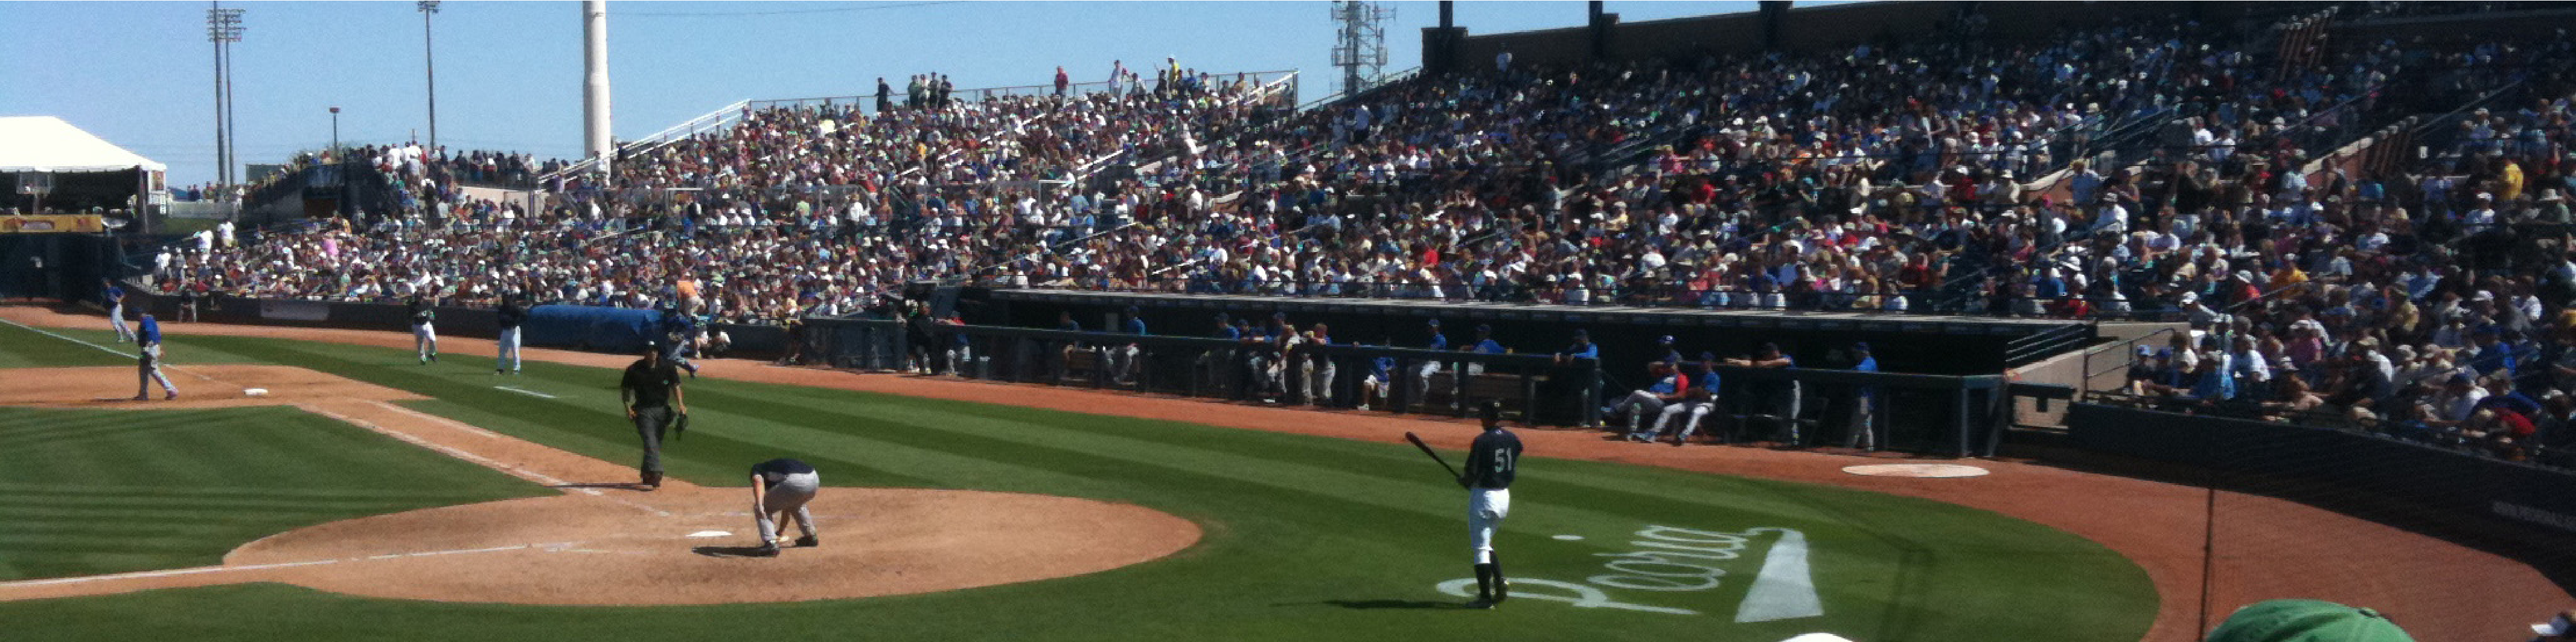
\includegraphics[width=\textwidth]{sampleteaser}
%   \caption{Seattle Mariners at Spring Training, 2010.}
%   \Description{Enjoying the baseball game from the third-base
%   seats. Ichiro Suzuki preparing to bat.}
%   \label{fig:teaser}
% \end{teaserfigure}

% \received{20 February 2007}
% \received[revised]{12 March 2009}
% \received[accepted]{5 June 2009}

%%
%% This command processes the author and affiliation and title
%% information and builds the first part of the formatted document.
\maketitle

% 
% introduction
% 

Named Entity informed Corpus Embedding (NEiCE), is a topic modeling algorithm that uses named entities (NE) to improve the quality of topics extracted from short-text content. The algorithm was introduced in the paper ``Topic Modeling on Podcast Short-Text Metadata'' by~\citet{valero2022topic} from Deezer Research. It is based on the CluWords~\cite{10.1145/3289600.3291032} algorithm, which clusters words based on their nearest neighbors. The authors claim that NeICE outperforms other topic modeling algorithms of the same class, such as Non-negative matrix factorization (NMF), Short-text topic modeling via non-negative matrix factorization (SeaNMF)~\cite{shi2018short} and Clustering words (CluWords)~\cite{10.1145/3289600.3291032}, on podcast metadata from Deezer, Spotify and iTunes.

We put the claims of the authors, regarding the performance of NEiCE on the 3 datasets, to the test and report our findings in this paper. We were able to successfully reproduce the results of the original paper with a few exceptions, which we will discuss in the following sections.

\section{Introduction}





% *algorithm survery / benchmark*

% - podcast metadata (title, description, etc.) are short
% - these algorithms deal with short data
% - studies show that NMF-based algorithms are better than probabilistic models on short text
% - NMF-based are more interpretable than neural models

% - **pseudo-documents-based**
%     - concatenate and use conventional algorithms
% - **probabilistic**
%     - generalized polya urna dirichlet multinomial mixture (GPU-DMM)
%         - https://dl.acm.org/doi/pdf/10.1145/2911451.2911499
% - **neural**
%     - Negative sampling and Quantization Topic Model (NQTM)
%         - https://aclanthology.org/2020.emnlp-main.138.pdf
%         - neural model
%         - quantification method to get peakier distributions for decoding
%         - better at discovering non-repetitive topics
% - **NMF-based**
%     - non-negative matrix factorization (NMF)
%         - https://citeseerx.ist.psu.edu/document?type=pdf&doi=f452c605e8ecf8cd3541ea7909d81d27deb08181
%         - decomposes term-document bag of words matrix into two low rank matrices
%         - first: document-topic representaiton matrix
%         - second: topic-term representaiton matrix 
%     - semantics assisted NMF (SeaNMF)
%         - https://dl.acm.org/doi/pdf/10.1145/3178876.3186009
%         - integrats word-context embeddings
%         - focuses on the learning
%     - clustering words (CluWords)
%         - https://dl.acm.org/doi/pdf/10.1145/3289600.3291032
%         - nearest neighbor search
%     - named entity informed corpus embedding (NEiCE)
%         - https://arxiv.org/pdf/2201.04419
%         - based on CluWords: https://dl.acm.org/doi/abs/10.1145/3289600.3291032
%         - named entity information in word embeddings from NMF
%         - NE makes sense because podcast metadata have a lot more named entities, and they are informative
%         - Wikipedia2Vec as embeddings

% ## methodology

% - $A$ has BoW representations for each document $\mathcal{D}$ and $K$ topics
%     - simple BoW matrix
% - factorization: $A \approx WH$
% - $W$ is the topic-term matrix: each row is a representation of a topic from the vocabulary $\mathcal{V}$
% - $H$ is the document-topic matrix: each row is a representation of a document from the topics

% *preprocessing*

% - identify named entities in title and description
% - link them to wikipedia entities using the "radboud entity linker" (REL) system
%     - detect NE mentions using "Flair", a named entity recognition (NER) system using embeddings
%     - find a unique candidate from list with wikipedia2vec
%     - return the Wikipedia page of a unique named entity with a confidence score that helps us to choose if we treat it as: a span of text, as a named entity, words to be processed seperately
% - clean vocabulary
%     - use NameDataset library to remove actors, athletes, etc. that are too common

% *computation*

% - apply NE-related re-weighting to the tf factor

% *datasets*

% - itunes: drop duplicate titles, drop if title and description together have less than 3 terms
% - spotify: drop duplicate titles, drop if title and description together have less than 3 terms, drop non-english podcasts (double check with "fastText", "CLD3")
% - deezer: largest
% - all have metadata (provided by creators), titles and descriptions, show name, in english-language
% - drop unpopular genres (< 300 shows)

% *evaluation*

% - common metrics for "topic coherence" for topic quality
% - normalized pointwise mutual information (NPMI) metric
%     - computed with "Palmetto" for each topic $k$ on wikipdeia
% - top words limit: 10
% - top topics limit: 20, 50, 100, 200
% - REL confidence threshold: 0.9
% - drop words that appear in less than 5 documents
% - remove stopwords using NLTK
% - default hyperparams for all models
% - original cluwords is evaluated on fastText and wikipedia2vec embeddings
% - neice config:
%     - alpha-word set to 0.34-0.4 because of cluwords (test range: 0.2, 0.3, 0.4, 0.5)
%     - alpha-ent set similarly
% - specs: Intel Xeon Gold 6134 CPU @ 3.20GHz with 32 cores and 128GB RAM

% ## results



% https://arxiv.org/pdf/2201.04419

\begin{table}[h]
  \centering
  \begin{tabular}{lrrrrrrrrrrrr}
      \toprule
      Dataset & \multicolumn{4}{c}{Deezer} & \multicolumn{4}{c}{Spotify} & \multicolumn{4}{c}{iTunes} \\
      & 20 & 50 & 100 & 200 & 20 & 50 & 100 & 200 & 20 & 50 & 100 & 200 \\
      \midrule
      NEiCE (0.2, 0.3) & 50.2 & 48.9 & 51.4 & 48.4 & 51.7 & 49.0 & 45.2 & 46.5 & 49.3 & 43.3 & 49.5 & 47.0 \\
      NEiCE (0.2, 0.4) & 53.1 & 49.2 & 50.8 & 50.6 & 48.7 & 48.7 & 43.5 & 41.7 & 47.2 & 49.5 & 50.7 & 51.3 \\
      NEiCE (0.3, 0.3) & 48.5 & 52.1 & 51.5 & 49.8 & 52.2 & 49.0 & 47.5 & 47.6 & 50.3 & 52.5 & 49.0 & 48.2 \\
      NEiCE (0.3, 0.4) & 53.3 & 50.9 & 55.3 & 51.6 & 50.1 & 48.5 & 51.1 & 49.8 & 52.5 & 49.5 & 49.2 & 49.8 \\
      NEiCE (0.4, 0.3) & 53.2 & 51.5 & 52.2 & 50.0 & 53.2 & 49.5 & 50.5 & 45.9 & 52.8 & 50.1 & 50.6 & 51.1 \\
      NEiCE (0.4, 0.4) & 56.4 & 52.6 & 48.1 & 49.0 & 51.0 & 48.2 & 47.3 & 47.8 & 52.4 & 51.9 & 49.9 & 47.4 \\
      NEiCE (0.5, 0.3) & 52.5 & 56.3 & 50.8 & 55.4 & 51.3 & 47.7 & 45.6 & 45.4 & 50.6 & 46.5 & 46.7 & 49.0 \\
      NEiCE (0.5, 0.4) & 56.3 & 60.6 & 54.9 & 53.3 & 55.0 & 49.9 & 46.7 & 45.0 & 50.5 & 52.0 & 48.7 & 46.1 \\
      \bottomrule
  \end{tabular}
  \caption{NEiCE dataset performance on Deezer, Spotify, and iTunes}
  \label{tab:neice-performance}
\end{table}







% # Experimental Setup

% <!-- steps necessary to reproduce results -->


% # evaluation loop

% run the eval loop `benchmark.sh` after a single iteration (as shown above) was successful.

% beware that the evaluation loop is very slow, with each cycle taking 100-600 seconds and around 2-3 days in total.

% ```bash
% chmod +x benchmark.sh
% ./benchmark.sh
% ```

% kudos to `@chrisizeh` and `@DennisToma` for providing inspiration (see: https://github.com/chrisizeh/podcast-topic-modeling)




% # patch notes

% ## patched

% - new dockerfile with dependency dump for reproducibility
% - added seeds to every file (random, numpy, torch, os), so a single iteration is sufficient for evaluation
% - changed `df.append(d, ignore_index=True)` to `pd.concat([df, pd.DataFrame([d])], ignore_index=True)` in `main_prepro.py` since the former is deprecated and disabled
% - fixed `data_preprocessing/utils.py`: path was relative to the script (not the working directory) and used linux path separators
% - fixed `data_preprocessing/utils.py` and `neice_model/wikipedia2vec_model.py`: replaced `get_feature_names` with `get_feature_names_out` to resolve `AttributeError` with `CountVectorizer`
% - fixed `neice_model.py`: replaced sklearn `NMF` argument `alpha` with `alpha_W` to resolve non existent parameter error

% ## unable to patch

% - note by authors: updated dependencies (REL, flairNLP) mean a different vocabulary. this makes it impossible to reproducible exact scores from original paper. however the distribution of scores should be similar.
% - spotify dataset not available since dec 2023 (https://podcastsdataset.byspotify.com/)
% - provided container:
%     - doesn't build
%         - the REL git dependency always pulls the latest commit, so it doesn't match the requirements.txt
%         - i took a commit from march 2022, when this paper was submitted
%     - not portable
%         - set arch emulation flag so it works on arm64
%     - needs gpu
%         - can't use docker in google colab due to cgroup configuration bug (there is no way to resolve this)
%         - chose CPU only implementation, rewrite container config
%     - needs to be run interactively
%         - fix with compose: `docker compose build && docker compose up -d && docker compose exec main echo 'done'`
%     - breaks on: `entity_linking/radboud_entity_linker_batch.py`:
%         - REL dependency missmatch: manually find and downgrade the right dependencies, freeze pip in container into `requirements.txt`
%         - flair NER model needs `SequenceTagger` wrapper and weights from Feb 26, 2021 commit on huggingface:
%             ```python
%             from flair.models import SequenceTagger
%             tagger_ner = SequenceTagger.load('flair/ner-english-fast@3d3d35790f78a00ef319939b9004209d1d05f788')
%             ```
%         - cryptic SQLite errors when calling `MentionDetection`, unable to patch → stopped using container provided in repository
% - virtualenv:
%     - almost worked, but `gcld3` doesn't build on arm64, even if you install the protobuf dependency → stopped using virtualenv, had to use docker or conda (chose docker)
% - the weights in `enwiki_20180420_300d.pkl` are not byte aligned which can throw segfaults when used with some of the libraries













%%
%% The acknowledgments section is defined using the "acks" environment
%% (and NOT an unnumbered section). This ensures the proper
%% identification of the section in the article metadata, and the
%% consistent spelling of the heading.
% \begin{acks}
% To Robert, for the bagels and explaining CMYK and color spaces.
% \end{acks}

%%
%% The next two lines define the bibliography style to be used, and
%% the bibliography file.
\bibliographystyle{ACM-Reference-Format}
\bibliography{sample-base}

%%
%% If your work has an appendix, this is the place to put it.
\appendix

\section{System Specifications}

All experiments were conducted on a consumer-grade laptop with the following specifications:

\begin{footnotesize}
\begin{verbatim}
$ system_profiler SPSoftwareDataType SPHardwareDataType
Software:

    System Software Overview:

      System Version: macOS 14.6.1 (23G93)
      Kernel Version: Darwin 23.6.0
      Boot Volume: Macintosh HD
      Boot Mode: Normal
      Computer Name: Yahya’s MacBook Pro
      User Name: Yahya Jabary (sueszli)
      Secure Virtual Memory: Enabled
      System Integrity Protection: Enabled
      Time since boot: 103 days, 2 hours, 59 minutes

Hardware:

    Hardware Overview:

      Model Name: MacBook Pro
      Model Identifier: Mac14,10
      Model Number: <redacted>
      Chip: Apple M2 Pro
      Total Number of Cores: 12 (8 performance and 4 efficiency)
      Memory: 16 GB
      System Firmware Version: 10151.140.19
      OS Loader Version: <redacted>
      Serial Number (system): <redacted>
      Hardware UUID: <redacted>
      Provisioning UDID: <redacted>
      Activation Lock Status: Disabled
\end{verbatim}
\end{footnotesize}

% \section{Results}

% The following shows the performance of the NEiCE algorithm on the Deezer and iTunes datasets, based on our reproduction of the original paper:

% \begin{tiny}
%     \begin{longtable}{|r|r|r|r|r|r|r|}
%     \caption{Performance of NEiCE algorithm on Deezer and iTunes datasets with different hyperparameters.}
%     \label{tab:neice-results} \\
    
%     \hline
%       $\alpha^{\text{ent}}$ & K & topics & neighbours & $\alpha^{\text{word}}$ & $C_v$ Deezer & $C_v$ iTunes \\
%       \hline

%       0.300000 & 20 & 10 & 5 & 0.200000 & 48.678100 & 51.668200 \\
%       0.300000 & 20 & 10 & 5 & 0.300000 & 48.678100 & 51.668200 \\
%       0.300000 & 20 & 10 & 5 & 0.400000 & 49.602300 & 50.995100 \\
%       0.300000 & 20 & 10 & 5 & 0.500000 & 49.856800 & 48.942800 \\
%       0.300000 & 20 & 10 & 10 & 0.200000 & 52.903800 & 51.369600 \\
%       0.300000 & 20 & 10 & 10 & 0.300000 & 52.903800 & 51.369600 \\
%       0.300000 & 20 & 10 & 10 & 0.400000 & 54.578000 & 52.581900 \\
%       0.300000 & 20 & 10 & 10 & 0.500000 & 52.162200 & 51.647200 \\
%       0.300000 & 20 & 10 & 20 & 0.200000 & 51.747600 & 51.406200 \\
%       0.300000 & 20 & 10 & 20 & 0.300000 & 51.747600 & 51.406200 \\
%       0.300000 & 20 & 10 & 20 & 0.400000 & 53.479300 & 50.824000 \\
%       0.300000 & 20 & 10 & 20 & 0.500000 & 54.610600 & 50.142200 \\
%       0.300000 & 20 & 10 & 500 & 0.200000 & 47.911800 & 51.432600 \\
%       0.300000 & 20 & 10 & 500 & 0.300000 & 49.932700 & 51.612300 \\
%       0.300000 & 20 & 10 & 500 & 0.400000 & 54.248100 & 51.327300 \\
%       0.300000 & 20 & 10 & 500 & 0.500000 & 54.707200 & 48.678400 \\
%       0.300000 & 20 & 20 & 5 & 0.200000 & 55.767100 & 52.914000 \\
%       0.300000 & 20 & 20 & 5 & 0.300000 & 55.767100 & 52.914000 \\
%       0.300000 & 20 & 20 & 5 & 0.400000 & 55.763200 & 53.290300 \\
%       0.300000 & 20 & 20 & 5 & 0.500000 & 54.566300 & 54.402700 \\
%       0.300000 & 20 & 20 & 10 & 0.200000 & 52.158100 & 53.345900 \\
%       0.300000 & 20 & 20 & 10 & 0.300000 & 53.193000 & 53.345900 \\
%       0.300000 & 20 & 20 & 10 & 0.400000 & 53.269400 & 53.678800 \\
%       0.300000 & 20 & 20 & 10 & 0.500000 & 54.643300 & 51.553200 \\
%       0.300000 & 20 & 20 & 20 & 0.200000 & 51.733400 & 52.204700 \\
%       0.300000 & 20 & 20 & 20 & 0.300000 & 51.733400 & 52.383100 \\
%       0.300000 & 20 & 20 & 20 & 0.400000 & 54.304200 & 52.234500 \\
%       0.300000 & 20 & 20 & 20 & 0.500000 & 54.124200 & 48.000500 \\
%       0.300000 & 20 & 20 & 500 & 0.200000 & 51.666700 & 49.951800 \\
%       0.300000 & 20 & 20 & 500 & 0.300000 & 52.286600 & 51.944400 \\
%       0.300000 & 20 & 20 & 500 & 0.400000 & 56.582000 & 51.427000 \\
%       0.300000 & 20 & 20 & 500 & 0.500000 & 54.785500 & 47.819600 \\
%       0.300000 & 20 & 50 & 5 & 0.200000 & 52.672100 & 47.632800 \\
%       0.300000 & 20 & 50 & 5 & 0.300000 & 52.672100 & 47.632800 \\
%       0.300000 & 20 & 50 & 5 & 0.400000 & 52.712400 & 51.010300 \\
%       0.300000 & 20 & 50 & 5 & 0.500000 & 53.813300 & 50.944500 \\
%       0.300000 & 20 & 50 & 10 & 0.200000 & 50.057900 & 50.086500 \\
%       0.300000 & 20 & 50 & 10 & 0.300000 & 49.858200 & 50.086500 \\
%       0.300000 & 20 & 50 & 10 & 0.400000 & 48.771600 & 51.152700 \\
%       0.300000 & 20 & 50 & 10 & 0.500000 & 50.314200 & 52.607900 \\
%       0.300000 & 20 & 50 & 20 & 0.200000 & 53.443200 & 53.011500 \\
%       0.300000 & 20 & 50 & 20 & 0.300000 & 53.443200 & 53.253700 \\
%       0.300000 & 20 & 50 & 20 & 0.400000 & 50.533900 & 52.991900 \\
%       0.300000 & 20 & 50 & 20 & 0.500000 & 49.297500 & 52.221500 \\
%       0.300000 & 20 & 50 & 500 & 0.200000 & 51.704500 & 49.561900 \\
%       0.300000 & 20 & 50 & 500 & 0.300000 & 55.033200 & 48.871800 \\
%       0.300000 & 20 & 50 & 500 & 0.400000 & 48.259000 & 53.130400 \\
%       0.300000 & 20 & 50 & 500 & 0.500000 & 52.332000 & 52.061500 \\
%       0.300000 & 20 & 100 & 5 & 0.200000 & 51.829100 & 48.920400 \\
%       0.300000 & 20 & 100 & 5 & 0.300000 & 51.829100 & 49.713300 \\
%       0.300000 & 20 & 100 & 5 & 0.400000 & 51.494700 & 49.306300 \\
%       0.300000 & 20 & 100 & 5 & 0.500000 & 53.377200 & 49.786100 \\
%       0.300000 & 20 & 100 & 10 & 0.200000 & 51.444100 & 51.927100 \\
%       0.300000 & 20 & 100 & 10 & 0.300000 & 51.754800 & 49.790900 \\
%       0.300000 & 20 & 100 & 10 & 0.400000 & 52.017900 & 53.001800 \\
%       0.300000 & 20 & 100 & 10 & 0.500000 & 53.971800 & 49.342100 \\
%       0.300000 & 20 & 100 & 20 & 0.200000 & 53.015000 & 53.215100 \\
%       0.300000 & 20 & 100 & 20 & 0.300000 & 50.462000 & 53.950300 \\
%       0.300000 & 20 & 100 & 20 & 0.400000 & 51.514500 & 51.655900 \\
%       0.300000 & 20 & 100 & 20 & 0.500000 & 49.549700 & 48.794500 \\
%       0.300000 & 20 & 100 & 500 & 0.200000 & 51.373300 & 50.877200 \\
%       0.300000 & 20 & 100 & 500 & 0.300000 & 49.996200 & 52.148000 \\
%       0.300000 & 20 & 100 & 500 & 0.400000 & 51.766200 & 51.128800 \\
%       0.300000 & 20 & 100 & 500 & 0.500000 & 49.028000 & 52.869400 \\
%       0.300000 & 50 & 10 & 5 & 0.200000 & 48.678100 & 51.668200 \\
%       0.300000 & 50 & 10 & 5 & 0.300000 & 48.678100 & 51.668200 \\
%       0.300000 & 50 & 10 & 5 & 0.400000 & 49.602300 & 50.995100 \\
%       0.300000 & 50 & 10 & 5 & 0.500000 & 49.856800 & 48.942800 \\
%       0.300000 & 50 & 10 & 10 & 0.200000 & 52.903800 & 51.369600 \\
%       0.300000 & 50 & 10 & 10 & 0.300000 & 52.903800 & 51.369600 \\
%       0.300000 & 50 & 10 & 10 & 0.400000 & 54.578000 & 52.581900 \\
%       0.300000 & 50 & 10 & 10 & 0.500000 & 52.162200 & 51.647200 \\
%       0.300000 & 50 & 10 & 20 & 0.200000 & 51.747600 & 51.406200 \\
%       0.300000 & 50 & 10 & 20 & 0.300000 & 51.747600 & 51.406200 \\
%       0.300000 & 50 & 10 & 20 & 0.400000 & 53.479300 & 50.824000 \\
%       0.300000 & 50 & 10 & 20 & 0.500000 & 54.610600 & 50.142200 \\
%       0.300000 & 50 & 10 & 500 & 0.200000 & 47.911800 & 51.432600 \\
%       0.300000 & 50 & 10 & 500 & 0.300000 & 49.932700 & 51.612300 \\
%       0.300000 & 50 & 10 & 500 & 0.400000 & 54.248100 & 51.327300 \\
%       0.300000 & 50 & 10 & 500 & 0.500000 & 54.707200 & 48.678400 \\
%       0.300000 & 50 & 20 & 5 & 0.200000 & 55.767100 & 52.914000 \\
%       0.300000 & 50 & 20 & 5 & 0.300000 & 55.767100 & 52.914000 \\
%       0.300000 & 50 & 20 & 5 & 0.400000 & 55.763200 & 53.290300 \\
%       0.300000 & 50 & 20 & 5 & 0.500000 & 54.566300 & 54.402700 \\
%       0.300000 & 50 & 20 & 10 & 0.200000 & 52.158100 & 53.345900 \\
%       0.300000 & 50 & 20 & 10 & 0.300000 & 53.193000 & 53.345900 \\
%       0.300000 & 50 & 20 & 10 & 0.400000 & 53.269400 & 53.678800 \\
%       0.300000 & 50 & 20 & 10 & 0.500000 & 54.643300 & 51.553200 \\
%       0.300000 & 50 & 20 & 20 & 0.200000 & 51.733400 & 52.204700 \\
%       0.300000 & 50 & 20 & 20 & 0.300000 & 51.733400 & 52.383100 \\
%       0.300000 & 50 & 20 & 20 & 0.400000 & 54.304200 & 52.234500 \\
%       0.300000 & 50 & 20 & 20 & 0.500000 & 54.124200 & 48.000500 \\
%       0.300000 & 50 & 20 & 500 & 0.200000 & 51.666700 & 49.951800 \\
%       0.300000 & 50 & 20 & 500 & 0.300000 & 52.286600 & 51.944400 \\
%       0.300000 & 50 & 20 & 500 & 0.400000 & 56.582000 & 51.427000 \\
%       0.300000 & 50 & 20 & 500 & 0.500000 & 54.785500 & 47.819600 \\
%       0.300000 & 50 & 50 & 5 & 0.200000 & 52.672100 & 47.632800 \\
%       0.300000 & 50 & 50 & 5 & 0.300000 & 52.672100 & 47.632800 \\
%       0.300000 & 50 & 50 & 5 & 0.400000 & 52.712400 & 51.010300 \\
%       0.300000 & 50 & 50 & 5 & 0.500000 & 53.813300 & 50.944500 \\
%       0.300000 & 50 & 50 & 10 & 0.200000 & 50.057900 & 50.086500 \\
%       0.300000 & 50 & 50 & 10 & 0.300000 & 49.858200 & 50.086500 \\
%       0.300000 & 50 & 50 & 10 & 0.400000 & 48.771600 & 51.152700 \\
%       0.300000 & 50 & 50 & 10 & 0.500000 & 50.314200 & 52.607900 \\
%       0.300000 & 50 & 50 & 20 & 0.200000 & 53.443200 & 53.011500 \\
%       0.300000 & 50 & 50 & 20 & 0.300000 & 53.443200 & 53.253700 \\
%       0.300000 & 50 & 50 & 20 & 0.400000 & 50.533900 & 52.991900 \\
%       0.300000 & 50 & 50 & 20 & 0.500000 & 49.297500 & 52.221500 \\
%       0.300000 & 50 & 50 & 500 & 0.200000 & 51.704500 & 49.561900 \\
%       0.300000 & 50 & 50 & 500 & 0.300000 & 55.033200 & 48.871800 \\
%       0.300000 & 50 & 50 & 500 & 0.400000 & 48.259000 & 53.130400 \\
%       0.300000 & 50 & 50 & 500 & 0.500000 & 52.332000 & 52.061500 \\
%       0.300000 & 50 & 100 & 5 & 0.200000 & 51.829100 & 48.920400 \\
%       0.300000 & 50 & 100 & 5 & 0.300000 & 51.829100 & 49.713300 \\
%       0.300000 & 50 & 100 & 5 & 0.400000 & 51.494700 & 49.306300 \\
%       0.300000 & 50 & 100 & 5 & 0.500000 & 53.377200 & 49.786100 \\
%       0.300000 & 50 & 100 & 10 & 0.200000 & 51.444100 & 51.927100 \\
%       0.300000 & 50 & 100 & 10 & 0.300000 & 51.754800 & 49.790900 \\
%       0.300000 & 50 & 100 & 10 & 0.400000 & 52.017900 & 53.001800 \\
%       0.300000 & 50 & 100 & 10 & 0.500000 & 53.971800 & 49.342100 \\
%       0.300000 & 50 & 100 & 20 & 0.200000 & 53.015000 & 53.215100 \\
%       0.300000 & 50 & 100 & 20 & 0.300000 & 50.462000 & 53.950300 \\
%       0.300000 & 50 & 100 & 20 & 0.400000 & 51.514500 & 51.655900 \\
%       0.300000 & 50 & 100 & 20 & 0.500000 & 49.549700 & 48.794500 \\
%       0.300000 & 50 & 100 & 500 & 0.200000 & 51.373300 & 50.877200 \\
%       0.300000 & 50 & 100 & 500 & 0.300000 & 49.996200 & 52.148000 \\
%       0.300000 & 50 & 100 & 500 & 0.400000 & 51.766200 & 51.128800 \\
%       0.300000 & 50 & 100 & 500 & 0.500000 & 49.028000 & 52.869400 \\
%       0.300000 & 100 & 10 & 5 & 0.200000 & 48.678100 & 51.668200 \\
%       0.300000 & 100 & 10 & 5 & 0.300000 & 48.678100 & 51.668200 \\
%       0.300000 & 100 & 10 & 5 & 0.400000 & 49.602300 & 50.995100 \\
%       0.300000 & 100 & 10 & 5 & 0.500000 & 49.856800 & 48.942800 \\
%       0.300000 & 100 & 10 & 10 & 0.200000 & 52.903800 & 51.369600 \\
%       0.300000 & 100 & 10 & 10 & 0.300000 & 52.903800 & 51.369600 \\
%       0.300000 & 100 & 10 & 10 & 0.400000 & 54.578000 & 52.581900 \\
%       0.300000 & 100 & 10 & 10 & 0.500000 & 52.162200 & 51.647200 \\
%       0.300000 & 100 & 10 & 20 & 0.200000 & 51.747600 & 51.406200 \\
%       0.300000 & 100 & 10 & 20 & 0.300000 & 51.747600 & 51.406200 \\
%       0.300000 & 100 & 10 & 20 & 0.400000 & 53.479300 & 50.824000 \\
%       0.300000 & 100 & 10 & 20 & 0.500000 & 54.610600 & 50.142200 \\
%       0.300000 & 100 & 10 & 500 & 0.200000 & 47.911800 & 51.432600 \\
%       0.300000 & 100 & 10 & 500 & 0.300000 & 49.932700 & 51.612300 \\
%       0.300000 & 100 & 10 & 500 & 0.400000 & 54.248100 & 51.327300 \\
%       0.300000 & 100 & 10 & 500 & 0.500000 & 54.707200 & 48.678400 \\
%       0.300000 & 100 & 20 & 5 & 0.200000 & 55.767100 & 52.914000 \\
%       0.300000 & 100 & 20 & 5 & 0.300000 & 55.767100 & 52.914000 \\
%       0.300000 & 100 & 20 & 5 & 0.400000 & 55.763200 & 53.290300 \\
%       0.300000 & 100 & 20 & 5 & 0.500000 & 54.566300 & 54.402700 \\
%       0.300000 & 100 & 20 & 10 & 0.200000 & 52.158100 & 53.345900 \\
%       0.300000 & 100 & 20 & 10 & 0.300000 & 53.193000 & 53.345900 \\
%       0.300000 & 100 & 20 & 10 & 0.400000 & 53.269400 & 53.678800 \\
%       0.300000 & 100 & 20 & 10 & 0.500000 & 54.643300 & 51.553200 \\
%       0.300000 & 100 & 20 & 20 & 0.200000 & 51.733400 & 52.204700 \\
%       0.300000 & 100 & 20 & 20 & 0.300000 & 51.733400 & 52.383100 \\
%       0.300000 & 100 & 20 & 20 & 0.400000 & 54.304200 & 52.234500 \\
%       0.300000 & 100 & 20 & 20 & 0.500000 & 54.124200 & 48.000500 \\
%       0.300000 & 100 & 20 & 500 & 0.200000 & 51.666700 & 49.951800 \\
%       0.300000 & 100 & 20 & 500 & 0.300000 & 52.286600 & 51.944400 \\
%       0.300000 & 100 & 20 & 500 & 0.400000 & 56.582000 & 51.427000 \\
%       0.300000 & 100 & 20 & 500 & 0.500000 & 54.785500 & 47.819600 \\
%       0.300000 & 100 & 50 & 5 & 0.200000 & 52.672100 & 47.632800 \\
%       0.300000 & 100 & 50 & 5 & 0.300000 & 52.672100 & 47.632800 \\
%       0.300000 & 100 & 50 & 5 & 0.400000 & 52.712400 & 51.010300 \\
%       0.300000 & 100 & 50 & 5 & 0.500000 & 53.813300 & 50.944500 \\
%       0.300000 & 100 & 50 & 10 & 0.200000 & 50.057900 & 50.086500 \\
%       0.300000 & 100 & 50 & 10 & 0.300000 & 49.858200 & 50.086500 \\
%       0.300000 & 100 & 50 & 10 & 0.400000 & 48.771600 & 51.152700 \\
%       0.300000 & 100 & 50 & 10 & 0.500000 & 50.314200 & 52.607900 \\
%       0.300000 & 100 & 50 & 20 & 0.200000 & 53.443200 & 53.011500 \\
%       0.300000 & 100 & 50 & 20 & 0.300000 & 53.443200 & 53.253700 \\
%       0.300000 & 100 & 50 & 20 & 0.400000 & 50.533900 & 52.991900 \\
%       0.300000 & 100 & 50 & 20 & 0.500000 & 49.297500 & 52.221500 \\
%       0.300000 & 100 & 50 & 500 & 0.200000 & 51.704500 & 49.561900 \\
%       0.300000 & 100 & 50 & 500 & 0.300000 & 55.033200 & 48.871800 \\
%       0.300000 & 100 & 50 & 500 & 0.400000 & 48.259000 & 53.130400 \\
%       0.300000 & 100 & 50 & 500 & 0.500000 & 52.332000 & 52.061500 \\
%       0.300000 & 100 & 100 & 5 & 0.200000 & 51.829100 & 48.920400 \\
%       0.300000 & 100 & 100 & 5 & 0.300000 & 51.829100 & 49.713300 \\
%       0.300000 & 100 & 100 & 5 & 0.400000 & 51.494700 & 49.306300 \\
%       0.300000 & 100 & 100 & 5 & 0.500000 & 53.377200 & 49.786100 \\
%       0.300000 & 100 & 100 & 10 & 0.200000 & 51.444100 & 51.927100 \\
%       0.300000 & 100 & 100 & 10 & 0.300000 & 51.754800 & 49.790900 \\
%       0.300000 & 100 & 100 & 10 & 0.400000 & 52.017900 & 53.001800 \\
%       0.300000 & 100 & 100 & 10 & 0.500000 & 53.971800 & 49.342100 \\
%       0.300000 & 100 & 100 & 20 & 0.200000 & 53.015000 & 53.215100 \\
%       0.300000 & 100 & 100 & 20 & 0.300000 & 50.462000 & 53.950300 \\
%       0.300000 & 100 & 100 & 20 & 0.400000 & 51.514500 & 51.655900 \\
%       0.300000 & 100 & 100 & 20 & 0.500000 & 49.549700 & 48.794500 \\
%       0.300000 & 100 & 100 & 500 & 0.200000 & 51.373300 & 50.877200 \\
%       0.300000 & 100 & 100 & 500 & 0.300000 & 49.996200 & 52.148000 \\
%       0.300000 & 100 & 100 & 500 & 0.400000 & 51.766200 & 51.128800 \\
%       0.300000 & 100 & 100 & 500 & 0.500000 & 49.028000 & 52.869400 \\
%       0.300000 & 200 & 10 & 5 & 0.200000 & 48.678100 & 51.668200 \\
%       0.300000 & 200 & 10 & 5 & 0.300000 & 48.678100 & 51.668200 \\
%       0.300000 & 200 & 10 & 5 & 0.400000 & 49.602300 & 50.995100 \\
%       0.300000 & 200 & 10 & 5 & 0.500000 & 49.856800 & 48.942800 \\
%       0.300000 & 200 & 10 & 10 & 0.200000 & 52.903800 & 51.369600 \\
%       0.300000 & 200 & 10 & 10 & 0.300000 & 52.903800 & 51.369600 \\
%       0.300000 & 200 & 10 & 10 & 0.400000 & 54.578000 & 52.581900 \\
%       0.300000 & 200 & 10 & 10 & 0.500000 & 52.162200 & 51.647200 \\
%       0.300000 & 200 & 10 & 20 & 0.200000 & 51.747600 & 51.406200 \\
%       0.300000 & 200 & 10 & 20 & 0.300000 & 51.747600 & 51.406200 \\
%       0.300000 & 200 & 10 & 20 & 0.400000 & 53.479300 & 50.824000 \\
%       0.300000 & 200 & 10 & 20 & 0.500000 & 54.610600 & 50.142200 \\
%       0.300000 & 200 & 10 & 500 & 0.200000 & 47.911800 & 51.432600 \\
%       0.300000 & 200 & 10 & 500 & 0.300000 & 49.932700 & 51.612300 \\
%       0.300000 & 200 & 10 & 500 & 0.400000 & 54.248100 & 51.327300 \\
%       0.300000 & 200 & 10 & 500 & 0.500000 & 54.707200 & 48.678400 \\
%       0.300000 & 200 & 20 & 5 & 0.200000 & 55.767100 & 52.914000 \\
%       0.300000 & 200 & 20 & 5 & 0.300000 & 55.767100 & 52.914000 \\
%       0.300000 & 200 & 20 & 5 & 0.400000 & 55.763200 & 53.290300 \\
%       0.300000 & 200 & 20 & 5 & 0.500000 & 54.566300 & 54.402700 \\
%       0.300000 & 200 & 20 & 10 & 0.200000 & 52.158100 & 53.345900 \\
%       0.300000 & 200 & 20 & 10 & 0.300000 & 53.193000 & 53.345900 \\
%       0.300000 & 200 & 20 & 10 & 0.400000 & 53.269400 & 53.678800 \\
%       0.300000 & 200 & 20 & 10 & 0.500000 & 54.643300 & 51.553200 \\
%       0.300000 & 200 & 20 & 20 & 0.200000 & 51.733400 & 52.204700 \\
%       0.300000 & 200 & 20 & 20 & 0.300000 & 51.733400 & 52.383100 \\
%       0.300000 & 200 & 20 & 20 & 0.400000 & 54.304200 & 52.234500 \\
%       0.300000 & 200 & 20 & 20 & 0.500000 & 54.124200 & 48.000500 \\
%       0.300000 & 200 & 20 & 500 & 0.200000 & 51.666700 & 49.951800 \\
%       0.300000 & 200 & 20 & 500 & 0.300000 & 52.286600 & 51.944400 \\
%       0.300000 & 200 & 20 & 500 & 0.400000 & 56.582000 & 51.427000 \\
%       0.300000 & 200 & 20 & 500 & 0.500000 & 54.785500 & 47.819600 \\
%       0.300000 & 200 & 50 & 5 & 0.200000 & 52.672100 & 47.632800 \\
%       0.300000 & 200 & 50 & 5 & 0.300000 & 52.672100 & 47.632800 \\
%       0.300000 & 200 & 50 & 5 & 0.400000 & 52.712400 & 51.010300 \\
%       0.300000 & 200 & 50 & 5 & 0.500000 & 53.813300 & 50.944500 \\
%       0.300000 & 200 & 50 & 10 & 0.200000 & 50.057900 & 50.086500 \\
%       0.300000 & 200 & 50 & 10 & 0.300000 & 49.858200 & 50.086500 \\
%       0.300000 & 200 & 50 & 10 & 0.400000 & 48.771600 & 51.152700 \\
%       0.300000 & 200 & 50 & 10 & 0.500000 & 50.314200 & 52.607900 \\
%       0.300000 & 200 & 50 & 20 & 0.200000 & 53.443200 & 53.011500 \\
%       0.300000 & 200 & 50 & 20 & 0.300000 & 53.443200 & 53.253700 \\
%       0.300000 & 200 & 50 & 20 & 0.400000 & 50.533900 & 52.991900 \\
%       0.300000 & 200 & 50 & 20 & 0.500000 & 49.297500 & 52.221500 \\
%       0.300000 & 200 & 50 & 500 & 0.200000 & 51.704500 & 49.561900 \\
%       0.300000 & 200 & 50 & 500 & 0.300000 & 55.033200 & 48.871800 \\
%       0.300000 & 200 & 50 & 500 & 0.400000 & 48.259000 & 53.130400 \\
%       0.300000 & 200 & 50 & 500 & 0.500000 & 52.332000 & 52.061500 \\
%       0.300000 & 200 & 100 & 5 & 0.200000 & 51.829100 & 48.920400 \\
%       0.300000 & 200 & 100 & 5 & 0.300000 & 51.829100 & 49.713300 \\
%       0.300000 & 200 & 100 & 5 & 0.400000 & 51.494700 & 49.306300 \\
%       0.300000 & 200 & 100 & 5 & 0.500000 & 53.377200 & 49.786100 \\
%       0.300000 & 200 & 100 & 10 & 0.200000 & 51.444100 & 51.927100 \\
%       0.300000 & 200 & 100 & 10 & 0.300000 & 51.754800 & 49.790900 \\
%       0.300000 & 200 & 100 & 10 & 0.400000 & 52.017900 & 53.001800 \\
%       0.300000 & 200 & 100 & 10 & 0.500000 & 53.971800 & 49.342100 \\
%       0.300000 & 200 & 100 & 20 & 0.200000 & 53.015000 & 53.215100 \\
%       0.300000 & 200 & 100 & 20 & 0.300000 & 50.462000 & 53.950300 \\
%       0.300000 & 200 & 100 & 20 & 0.400000 & 51.514500 & 51.655900 \\
%       0.300000 & 200 & 100 & 20 & 0.500000 & 49.549700 & 48.794500 \\
%       0.300000 & 200 & 100 & 500 & 0.200000 & 51.373300 & 50.877200 \\
%       0.300000 & 200 & 100 & 500 & 0.300000 & 49.996200 & 52.148000 \\
%       0.300000 & 200 & 100 & 500 & 0.400000 & 51.766200 & 51.128800 \\
%       0.300000 & 200 & 100 & 500 & 0.500000 & 49.028000 & 52.869400 \\
%       0.400000 & 20 & 10 & 5 & 0.200000 & 48.678100 & 51.668200 \\
%       0.400000 & 20 & 10 & 5 & 0.300000 & 48.678100 & 51.668200 \\
%       0.400000 & 20 & 10 & 5 & 0.400000 & 49.602300 & 50.995100 \\
%       0.400000 & 20 & 10 & 5 & 0.500000 & 49.856800 & 48.942800 \\
%       0.400000 & 20 & 10 & 10 & 0.200000 & 52.903800 & 51.369600 \\
%       0.400000 & 20 & 10 & 10 & 0.300000 & 52.903800 & 51.369600 \\
%       0.400000 & 20 & 10 & 10 & 0.400000 & 54.578000 & 52.581900 \\
%       0.400000 & 20 & 10 & 10 & 0.500000 & 52.162200 & 51.647200 \\
%       0.400000 & 20 & 10 & 20 & 0.200000 & 51.747600 & 51.406200 \\
%       0.400000 & 20 & 10 & 20 & 0.300000 & 51.747600 & 51.406200 \\
%       0.400000 & 20 & 10 & 20 & 0.400000 & 53.479300 & 50.824000 \\
%       0.400000 & 20 & 10 & 20 & 0.500000 & 54.610600 & 50.142200 \\
%       0.400000 & 20 & 10 & 500 & 0.200000 & 47.911800 & 51.432600 \\
%       0.400000 & 20 & 10 & 500 & 0.300000 & 49.932700 & 51.612300 \\
%       0.400000 & 20 & 10 & 500 & 0.400000 & 54.248100 & 51.327300 \\
%       0.400000 & 20 & 10 & 500 & 0.500000 & 54.707200 & 48.678400 \\
%       0.400000 & 20 & 20 & 5 & 0.200000 & 55.767100 & 52.914000 \\
%       0.400000 & 20 & 20 & 5 & 0.300000 & 55.767100 & 52.914000 \\
%       0.400000 & 20 & 20 & 5 & 0.400000 & 55.763200 & 53.290300 \\
%       0.400000 & 20 & 20 & 5 & 0.500000 & 54.566300 & NaN \\
%       0.400000 & 20 & 20 & 10 & 0.200000 & 52.158100 & 53.345900 \\
%       0.400000 & 20 & 20 & 10 & 0.300000 & 53.193000 & 53.345900 \\
%       0.400000 & 20 & 20 & 10 & 0.400000 & 53.269400 & 53.678800 \\
%       0.400000 & 20 & 20 & 10 & 0.500000 & 54.643300 & 51.553200 \\
%       0.400000 & 20 & 20 & 20 & 0.200000 & 51.733400 & 52.204700 \\
%       0.400000 & 20 & 20 & 20 & 0.300000 & 51.733400 & 52.383100 \\
%       0.400000 & 20 & 20 & 20 & 0.400000 & 54.304200 & 52.234500 \\
%       0.400000 & 20 & 20 & 20 & 0.500000 & 54.124200 & 48.000500 \\
%       0.400000 & 20 & 20 & 500 & 0.200000 & 51.666700 & 49.951800 \\
%       0.400000 & 20 & 20 & 500 & 0.300000 & 52.286600 & 51.944400 \\
%       0.400000 & 20 & 20 & 500 & 0.400000 & 56.582000 & 51.427000 \\
%       0.400000 & 20 & 20 & 500 & 0.500000 & 54.785500 & 47.819600 \\
%       0.400000 & 20 & 50 & 5 & 0.200000 & 52.672100 & 47.632800 \\
%       0.400000 & 20 & 50 & 5 & 0.300000 & 52.672100 & 47.632800 \\
%       0.400000 & 20 & 50 & 5 & 0.400000 & 52.712400 & 51.010300 \\
%       0.400000 & 20 & 50 & 5 & 0.500000 & 53.813300 & 50.944500 \\
%       0.400000 & 20 & 50 & 10 & 0.200000 & 50.057900 & 50.086500 \\
%       0.400000 & 20 & 50 & 10 & 0.300000 & 49.858200 & 50.086500 \\
%       0.400000 & 20 & 50 & 10 & 0.400000 & 48.771600 & 51.152700 \\
%       0.400000 & 20 & 50 & 10 & 0.500000 & 50.314200 & 52.607900 \\
%       0.400000 & 20 & 50 & 20 & 0.200000 & 53.443200 & 53.011500 \\
%       0.400000 & 20 & 50 & 20 & 0.300000 & 53.443200 & 53.253700 \\
%       0.400000 & 20 & 50 & 20 & 0.400000 & 50.533900 & 52.991900 \\
%       0.400000 & 20 & 50 & 20 & 0.500000 & 49.297500 & 52.221500 \\
%       0.400000 & 20 & 50 & 500 & 0.200000 & 51.704500 & 49.561900 \\
%       0.400000 & 20 & 50 & 500 & 0.300000 & 55.033200 & 48.871800 \\
%       0.400000 & 20 & 50 & 500 & 0.400000 & 48.259000 & 53.130400 \\
%       0.400000 & 20 & 50 & 500 & 0.500000 & 52.332000 & 52.061500 \\
%       0.400000 & 20 & 100 & 5 & 0.200000 & 51.829100 & 48.920400 \\
%       0.400000 & 20 & 100 & 5 & 0.300000 & 51.829100 & 49.713300 \\
%       0.400000 & 20 & 100 & 5 & 0.400000 & 51.494700 & 49.306300 \\
%       0.400000 & 20 & 100 & 5 & 0.500000 & 53.377200 & 49.786100 \\
%       0.400000 & 20 & 100 & 10 & 0.200000 & 51.444100 & 51.927100 \\
%       0.400000 & 20 & 100 & 10 & 0.300000 & 51.754800 & 49.790900 \\
%       0.400000 & 20 & 100 & 10 & 0.400000 & 52.017900 & 53.001800 \\
%       0.400000 & 20 & 100 & 10 & 0.500000 & 53.971800 & 49.342100 \\
%       0.400000 & 20 & 100 & 20 & 0.200000 & 53.015000 & 53.215100 \\
%       0.400000 & 20 & 100 & 20 & 0.300000 & 50.462000 & 53.950300 \\
%       0.400000 & 20 & 100 & 20 & 0.400000 & 51.514500 & 51.655900 \\
%       0.400000 & 20 & 100 & 20 & 0.500000 & 49.549700 & 48.794500 \\
%       0.400000 & 20 & 100 & 500 & 0.200000 & 51.373300 & 50.877200 \\
%       0.400000 & 20 & 100 & 500 & 0.300000 & 49.996200 & 52.148000 \\
%       0.400000 & 20 & 100 & 500 & 0.400000 & 51.766200 & 51.128800 \\
%       0.400000 & 20 & 100 & 500 & 0.500000 & 49.028000 & 52.869400 \\
%       0.400000 & 50 & 10 & 5 & 0.200000 & 48.678100 & 51.668200 \\
%       0.400000 & 50 & 10 & 5 & 0.300000 & 48.678100 & 51.668200 \\
%       0.400000 & 50 & 10 & 5 & 0.400000 & 49.602300 & 50.995100 \\
%       0.400000 & 50 & 10 & 5 & 0.500000 & 49.856800 & 48.942800 \\
%       0.400000 & 50 & 10 & 10 & 0.200000 & 52.903800 & 51.369600 \\
%       0.400000 & 50 & 10 & 10 & 0.300000 & 52.903800 & 51.369600 \\
%       0.400000 & 50 & 10 & 10 & 0.400000 & 54.578000 & 52.581900 \\
%       0.400000 & 50 & 10 & 10 & 0.500000 & 52.162200 & 51.647200 \\
%       0.400000 & 50 & 10 & 20 & 0.200000 & 51.747600 & 51.406200 \\
%       0.400000 & 50 & 10 & 20 & 0.300000 & 51.747600 & 51.406200 \\
%       0.400000 & 50 & 10 & 20 & 0.400000 & 53.479300 & 50.824000 \\
%       0.400000 & 50 & 10 & 20 & 0.500000 & 54.610600 & 50.142200 \\
%       0.400000 & 50 & 10 & 500 & 0.200000 & 47.911800 & 51.432600 \\
%       0.400000 & 50 & 10 & 500 & 0.300000 & 49.932700 & 51.612300 \\
%       0.400000 & 50 & 10 & 500 & 0.400000 & 54.248100 & 51.327300 \\
%       0.400000 & 50 & 10 & 500 & 0.500000 & 54.707200 & 48.678400 \\
%       0.400000 & 50 & 20 & 5 & 0.200000 & 55.767100 & 52.914000 \\
%       0.400000 & 50 & 20 & 5 & 0.300000 & 55.767100 & 52.914000 \\
%       0.400000 & 50 & 20 & 5 & 0.400000 & 55.763200 & 53.290300 \\
%       0.400000 & 50 & 20 & 5 & 0.500000 & 54.566300 & 54.402700 \\
%       0.400000 & 50 & 20 & 10 & 0.200000 & 52.158100 & 53.345900 \\
%       0.400000 & 50 & 20 & 10 & 0.300000 & 53.193000 & 53.345900 \\
%       0.400000 & 50 & 20 & 10 & 0.400000 & 53.269400 & 53.678800 \\
%       0.400000 & 50 & 20 & 10 & 0.500000 & 54.643300 & 51.553200 \\
%       0.400000 & 50 & 20 & 20 & 0.200000 & 51.733400 & 52.204700 \\
%       0.400000 & 50 & 20 & 20 & 0.300000 & 51.733400 & 52.383100 \\
%       0.400000 & 50 & 20 & 20 & 0.400000 & 54.304200 & 52.234500 \\
%       0.400000 & 50 & 20 & 20 & 0.500000 & 54.124200 & 48.000500 \\
%       0.400000 & 50 & 20 & 500 & 0.200000 & 51.666700 & 49.951800 \\
%       0.400000 & 50 & 20 & 500 & 0.300000 & 52.286600 & 51.944400 \\
%       0.400000 & 50 & 20 & 500 & 0.400000 & 56.582000 & 51.427000 \\
%       0.400000 & 50 & 20 & 500 & 0.500000 & 54.785500 & 47.819600 \\
%       0.400000 & 50 & 50 & 5 & 0.200000 & 52.672100 & 47.632800 \\
%       0.400000 & 50 & 50 & 5 & 0.300000 & 52.672100 & 47.632800 \\
%       0.400000 & 50 & 50 & 5 & 0.400000 & 52.712400 & 51.010300 \\
%       0.400000 & 50 & 50 & 5 & 0.500000 & 53.813300 & 50.944500 \\
%       0.400000 & 50 & 50 & 10 & 0.200000 & 50.057900 & 50.086500 \\
%       0.400000 & 50 & 50 & 10 & 0.300000 & 49.858200 & 50.086500 \\
%       0.400000 & 50 & 50 & 10 & 0.400000 & 48.771600 & 51.152700 \\
%       0.400000 & 50 & 50 & 10 & 0.500000 & 50.314200 & 52.607900 \\
%       0.400000 & 50 & 50 & 20 & 0.200000 & 53.443200 & 53.011500 \\
%       0.400000 & 50 & 50 & 20 & 0.300000 & 53.443200 & 53.253700 \\
%       0.400000 & 50 & 50 & 20 & 0.400000 & 50.533900 & 52.991900 \\
%       0.400000 & 50 & 50 & 20 & 0.500000 & 49.297500 & 52.221500 \\
%       0.400000 & 50 & 50 & 500 & 0.200000 & 51.704500 & 49.561900 \\
%       0.400000 & 50 & 50 & 500 & 0.300000 & 55.033200 & 48.871800 \\
%       0.400000 & 50 & 50 & 500 & 0.400000 & 48.259000 & 53.130400 \\
%       0.400000 & 50 & 50 & 500 & 0.500000 & 52.332000 & 52.061500 \\
%       0.400000 & 50 & 100 & 5 & 0.200000 & 51.829100 & 48.920400 \\
%       0.400000 & 50 & 100 & 5 & 0.300000 & 51.829100 & 49.713300 \\
%       0.400000 & 50 & 100 & 5 & 0.400000 & 51.494700 & 49.306300 \\
%       0.400000 & 50 & 100 & 5 & 0.500000 & 53.377200 & 49.786100 \\
%       0.400000 & 50 & 100 & 10 & 0.200000 & 51.444100 & 51.927100 \\
%       0.400000 & 50 & 100 & 10 & 0.300000 & 51.754800 & 49.790900 \\
%       0.400000 & 50 & 100 & 10 & 0.400000 & 52.017900 & 53.001800 \\
%       0.400000 & 50 & 100 & 10 & 0.500000 & 53.971800 & 49.342100 \\
%       0.400000 & 50 & 100 & 20 & 0.200000 & 53.015000 & 53.215100 \\
%       0.400000 & 50 & 100 & 20 & 0.300000 & 50.462000 & 53.950300 \\
%       0.400000 & 50 & 100 & 20 & 0.400000 & 51.514500 & 51.655900 \\
%       0.400000 & 50 & 100 & 20 & 0.500000 & 49.549700 & 48.794500 \\
%       0.400000 & 50 & 100 & 500 & 0.200000 & 51.373300 & 50.877200 \\
%       0.400000 & 50 & 100 & 500 & 0.300000 & 49.996200 & 52.148000 \\
%       0.400000 & 50 & 100 & 500 & 0.400000 & 51.766200 & 51.128800 \\
%       0.400000 & 50 & 100 & 500 & 0.500000 & 49.028000 & 52.869400 \\
%       0.400000 & 100 & 10 & 5 & 0.200000 & 48.678100 & 51.668200 \\
%       0.400000 & 100 & 10 & 5 & 0.300000 & 48.678100 & 51.668200 \\
%       0.400000 & 100 & 10 & 5 & 0.400000 & 49.602300 & 50.995100 \\
%       0.400000 & 100 & 10 & 5 & 0.500000 & 49.856800 & 48.942800 \\
%       0.400000 & 100 & 10 & 10 & 0.200000 & 52.903800 & 51.369600 \\
%       0.400000 & 100 & 10 & 10 & 0.300000 & 52.903800 & 51.369600 \\
%       0.400000 & 100 & 10 & 10 & 0.400000 & 54.578000 & 52.581900 \\
%       0.400000 & 100 & 10 & 10 & 0.500000 & 52.162200 & 51.647200 \\
%       0.400000 & 100 & 10 & 20 & 0.200000 & 51.747600 & 51.406200 \\
%       0.400000 & 100 & 10 & 20 & 0.300000 & 51.747600 & 51.406200 \\
%       0.400000 & 100 & 10 & 20 & 0.400000 & 53.479300 & 50.824000 \\
%       0.400000 & 100 & 10 & 20 & 0.500000 & 54.610600 & 50.142200 \\
%       0.400000 & 100 & 10 & 500 & 0.200000 & 47.911800 & 51.432600 \\
%       0.400000 & 100 & 10 & 500 & 0.300000 & 49.932700 & 51.612300 \\
%       0.400000 & 100 & 10 & 500 & 0.400000 & 54.248100 & 51.327300 \\
%       0.400000 & 100 & 10 & 500 & 0.500000 & 54.707200 & 48.678400 \\
%       0.400000 & 100 & 20 & 5 & 0.200000 & 55.767100 & 52.914000 \\
%       0.400000 & 100 & 20 & 5 & 0.300000 & 55.767100 & 52.914000 \\
%       0.400000 & 100 & 20 & 5 & 0.400000 & 55.763200 & 53.290300 \\
%       0.400000 & 100 & 20 & 5 & 0.500000 & 54.566300 & 54.402700 \\
%       0.400000 & 100 & 20 & 10 & 0.200000 & 52.158100 & 53.345900 \\
%       0.400000 & 100 & 20 & 10 & 0.300000 & 53.193000 & 53.345900 \\
%       0.400000 & 100 & 20 & 10 & 0.400000 & 53.269400 & 53.678800 \\
%       0.400000 & 100 & 20 & 10 & 0.500000 & 54.643300 & 51.553200 \\
%       0.400000 & 100 & 20 & 20 & 0.200000 & 51.733400 & 52.204700 \\
%       0.400000 & 100 & 20 & 20 & 0.300000 & 51.733400 & 52.383100 \\
%       0.400000 & 100 & 20 & 20 & 0.400000 & 54.304200 & 52.234500 \\
%       0.400000 & 100 & 20 & 20 & 0.500000 & 54.124200 & 48.000500 \\
%       0.400000 & 100 & 20 & 500 & 0.200000 & 51.666700 & 49.951800 \\
%       0.400000 & 100 & 20 & 500 & 0.300000 & 52.286600 & 51.944400 \\
%       0.400000 & 100 & 20 & 500 & 0.400000 & 56.582000 & 51.427000 \\
%       0.400000 & 100 & 20 & 500 & 0.500000 & 54.785500 & 47.819600 \\
%       0.400000 & 100 & 50 & 5 & 0.200000 & 52.672100 & 47.632800 \\
%       0.400000 & 100 & 50 & 5 & 0.300000 & 52.672100 & 47.632800 \\
%       0.400000 & 100 & 50 & 5 & 0.400000 & 52.712400 & 51.010300 \\
%       0.400000 & 100 & 50 & 5 & 0.500000 & 53.813300 & 50.944500 \\
%       0.400000 & 100 & 50 & 10 & 0.200000 & 50.057900 & 50.086500 \\
%       0.400000 & 100 & 50 & 10 & 0.300000 & 49.858200 & 50.086500 \\
%       0.400000 & 100 & 50 & 10 & 0.400000 & 48.771600 & 51.152700 \\
%       0.400000 & 100 & 50 & 10 & 0.500000 & 50.314200 & 52.607900 \\
%       0.400000 & 100 & 50 & 20 & 0.200000 & 53.443200 & 53.011500 \\
%       0.400000 & 100 & 50 & 20 & 0.300000 & 53.443200 & 53.253700 \\
%       0.400000 & 100 & 50 & 20 & 0.400000 & 50.533900 & 52.991900 \\
%       0.400000 & 100 & 50 & 20 & 0.500000 & 49.297500 & 52.221500 \\
%       0.400000 & 100 & 50 & 500 & 0.200000 & 51.704500 & 49.561900 \\
%       0.400000 & 100 & 50 & 500 & 0.300000 & 55.033200 & 48.871800 \\
%       0.400000 & 100 & 50 & 500 & 0.400000 & 48.259000 & 53.130400 \\
%       0.400000 & 100 & 50 & 500 & 0.500000 & 52.332000 & 52.061500 \\
%       0.400000 & 100 & 100 & 5 & 0.200000 & 51.829100 & 48.920400 \\
%       0.400000 & 100 & 100 & 5 & 0.300000 & 51.829100 & 49.713300 \\
%       0.400000 & 100 & 100 & 5 & 0.400000 & 51.494700 & 49.306300 \\
%       0.400000 & 100 & 100 & 5 & 0.500000 & 53.377200 & 49.786100 \\
%       0.400000 & 100 & 100 & 10 & 0.200000 & 51.444100 & 51.927100 \\
%       0.400000 & 100 & 100 & 10 & 0.300000 & 51.754800 & 49.790900 \\
%       0.400000 & 100 & 100 & 10 & 0.400000 & 52.017900 & 53.001800 \\
%       0.400000 & 100 & 100 & 10 & 0.500000 & 53.971800 & 49.342100 \\
%       0.400000 & 100 & 100 & 20 & 0.200000 & 53.015000 & 53.215100 \\
%       0.400000 & 100 & 100 & 20 & 0.300000 & 50.462000 & 53.950300 \\
%       0.400000 & 100 & 100 & 20 & 0.400000 & 51.514500 & 51.655900 \\
%       0.400000 & 100 & 100 & 20 & 0.500000 & 49.549700 & 48.794500 \\
%       0.400000 & 100 & 100 & 500 & 0.200000 & 51.373300 & 50.877200 \\
%       0.400000 & 100 & 100 & 500 & 0.300000 & 49.996200 & 52.148000 \\
%       0.400000 & 100 & 100 & 500 & 0.400000 & 51.766200 & 51.128800 \\
%       0.400000 & 100 & 100 & 500 & 0.500000 & 49.028000 & 52.869400 \\
%       0.400000 & 200 & 10 & 5 & 0.200000 & 48.678100 & 51.668200 \\
%       0.400000 & 200 & 10 & 5 & 0.300000 & 48.678100 & 51.668200 \\
%       0.400000 & 200 & 10 & 5 & 0.400000 & 49.602300 & 50.995100 \\
%       0.400000 & 200 & 10 & 5 & 0.500000 & 49.856800 & 48.942800 \\
%       0.400000 & 200 & 10 & 10 & 0.200000 & 52.903800 & 51.369600 \\
%       0.400000 & 200 & 10 & 10 & 0.300000 & 52.903800 & 51.369600 \\
%       0.400000 & 200 & 10 & 10 & 0.400000 & 54.578000 & 52.581900 \\
%       0.400000 & 200 & 10 & 10 & 0.500000 & 52.162200 & 51.647200 \\
%       0.400000 & 200 & 10 & 20 & 0.200000 & 51.747600 & 51.406200 \\
%       0.400000 & 200 & 10 & 20 & 0.300000 & 51.747600 & 51.406200 \\
%       0.400000 & 200 & 10 & 20 & 0.400000 & 53.479300 & 50.824000 \\
%       0.400000 & 200 & 10 & 20 & 0.500000 & 54.610600 & 50.142200 \\
%       0.400000 & 200 & 10 & 500 & 0.200000 & 47.911800 & 51.432600 \\
%       0.400000 & 200 & 10 & 500 & 0.300000 & 49.932700 & 51.612300 \\
%       0.400000 & 200 & 10 & 500 & 0.400000 & 54.248100 & 51.327300 \\
%       0.400000 & 200 & 10 & 500 & 0.500000 & 54.707200 & 48.678400 \\
%       0.400000 & 200 & 20 & 5 & 0.200000 & 55.767100 & 52.914000 \\
%       0.400000 & 200 & 20 & 5 & 0.300000 & 55.767100 & 52.914000 \\
%       0.400000 & 200 & 20 & 5 & 0.400000 & 55.763200 & 53.290300 \\
%       0.400000 & 200 & 20 & 5 & 0.500000 & 54.566300 & 54.402700 \\
%       0.400000 & 200 & 20 & 10 & 0.200000 & 52.158100 & 53.345900 \\
%       0.400000 & 200 & 20 & 10 & 0.300000 & 53.193000 & 53.345900 \\
%       0.400000 & 200 & 20 & 10 & 0.400000 & 53.269400 & 53.678800 \\
%       0.400000 & 200 & 20 & 10 & 0.500000 & 54.643300 & 51.553200 \\
%       0.400000 & 200 & 20 & 20 & 0.200000 & 51.733400 & 52.204700 \\
%       0.400000 & 200 & 20 & 20 & 0.300000 & 51.733400 & 52.383100 \\
%       0.400000 & 200 & 20 & 20 & 0.400000 & 54.304200 & 52.234500 \\
%       0.400000 & 200 & 20 & 20 & 0.500000 & 54.124200 & 48.000500 \\
%       0.400000 & 200 & 20 & 500 & 0.200000 & 51.666700 & 49.951800 \\
%       0.400000 & 200 & 20 & 500 & 0.300000 & 52.286600 & 51.944400 \\
%       0.400000 & 200 & 20 & 500 & 0.400000 & 56.582000 & 51.427000 \\
%       0.400000 & 200 & 20 & 500 & 0.500000 & 54.785500 & 47.819600 \\
%       0.400000 & 200 & 50 & 5 & 0.200000 & 52.672100 & 47.632800 \\
%       0.400000 & 200 & 50 & 5 & 0.300000 & 52.672100 & 47.632800 \\
%       0.400000 & 200 & 50 & 5 & 0.400000 & 52.712400 & 51.010300 \\
%       0.400000 & 200 & 50 & 5 & 0.500000 & 53.813300 & 50.944500 \\
%       0.400000 & 200 & 50 & 10 & 0.200000 & 50.057900 & 50.086500 \\
%       0.400000 & 200 & 50 & 10 & 0.300000 & 49.858200 & 50.086500 \\
%       0.400000 & 200 & 50 & 10 & 0.400000 & 48.771600 & 51.152700 \\
%       0.400000 & 200 & 50 & 10 & 0.500000 & 50.314200 & 52.607900 \\
%       0.400000 & 200 & 50 & 20 & 0.200000 & 53.443200 & 53.011500 \\
%       0.400000 & 200 & 50 & 20 & 0.300000 & 53.443200 & 53.253700 \\
%       0.400000 & 200 & 50 & 20 & 0.400000 & 50.533900 & 52.991900 \\
%       0.400000 & 200 & 50 & 20 & 0.500000 & 49.297500 & 52.221500 \\
%       0.400000 & 200 & 50 & 500 & 0.200000 & 51.704500 & 49.561900 \\
%       0.400000 & 200 & 50 & 500 & 0.300000 & 55.033200 & 48.871800 \\
%       0.400000 & 200 & 50 & 500 & 0.400000 & 48.259000 & 53.130400 \\
%       0.400000 & 200 & 50 & 500 & 0.500000 & 52.332000 & 52.061500 \\
%       0.400000 & 200 & 100 & 5 & 0.200000 & 51.829100 & 48.920400 \\
%       0.400000 & 200 & 100 & 5 & 0.300000 & 51.829100 & 49.713300 \\
%       0.400000 & 200 & 100 & 5 & 0.400000 & 51.494700 & 49.306300 \\
%       0.400000 & 200 & 100 & 5 & 0.500000 & 53.377200 & 49.786100 \\
%       0.400000 & 200 & 100 & 10 & 0.200000 & 51.444100 & 51.927100 \\
%       0.400000 & 200 & 100 & 10 & 0.300000 & 51.754800 & 49.790900 \\
%       0.400000 & 200 & 100 & 10 & 0.400000 & 52.017900 & 53.001800 \\
%       0.400000 & 200 & 100 & 10 & 0.500000 & 53.971800 & 49.342100 \\
%       0.400000 & 200 & 100 & 20 & 0.200000 & 53.015000 & 53.215100 \\
%       0.400000 & 200 & 100 & 20 & 0.300000 & 50.462000 & 53.950300 \\
%       0.400000 & 200 & 100 & 20 & 0.400000 & 51.514500 & 51.655900 \\
%       0.400000 & 200 & 100 & 20 & 0.500000 & 49.549700 & 48.794500 \\
%       0.400000 & 200 & 100 & 500 & 0.200000 & 51.373300 & 50.877200 \\
%       0.400000 & 200 & 100 & 500 & 0.300000 & 49.996200 & 52.148000 \\
%       0.400000 & 200 & 100 & 500 & 0.400000 & 51.766200 & 51.128800 \\
%       0.400000 & 200 & 100 & 500 & 0.500000 & 49.028000 & 52.869400 \\
%       \hline
%   \end{longtable}
% \end{tiny}

\end{document}
\endinput
%%
%% End of file `sample-sigconf.tex'.
